\documentclass{article}

\newif\ifhighlightnew\highlightnewfalse

\usepackage{amsmath}
\usepackage{amssymb}
\usepackage{amsthm}
\usepackage{bcprules}
\usepackage{stmaryrd}
\usepackage{xspace}
\usepackage[table]{xcolor}
\usepackage{tikz}
\usetikzlibrary{chains,positioning}

\tikzstyle{history}=[on chain,join,circle,fill]

\newtheorem{definition}{Definition}
\newtheorem{theorem}{Theorem}
\newcommand{\yes}{\cellcolor{green!30}yes}
\newcommand{\no}{\cellcolor{red!20}no}
\newcommand{\maybe}{\cellcolor{orange!70!yellow!40}maybe}
\renewcommand{\partial}{\cellcolor{yellow!30}partial}
\newcommand{\mbf}[1]{\ensuremath{\mathbf{#1}}}

% \mbfbe takes four arguments:
% 1. some text to put before a keyword
% 2. some text to put after a keyword
% 3. a prefix
% 4. a keyword
% It then generates a new latex command of the form \<prefix><keyword> that
% will print that keyword in a boldface font with some text before and after
% it. For example, \mbfbe{foo\ }{\ bar}{com}{foreach} will define a command
% \comforeach that expands to {foo\ \ensuremath{\mathbf{foreach}}\ bar}.

\newcommand{\mbfbe}[4]{\expandafter\newcommand\csname #3#4\endcsname{#1\mbf{#4}#2}}
\newcommand{\exspace}{\mbfbe{}\xspace{}}
\newcommand{\eexspace}{\mbfbe{}\xspace{e}}
\newcommand{\eespace}{\mbfbe{}\ {e}}
\newcommand{\bespace}{\mbfbe\ \ {}}
\newcommand{\ebespace}{\mbfbe\ \ {e}}
\newcommand{\kexspace}{\mbfbe{}\xspace{k}}

\newcommand{\undefined}{\ensuremath{\bot}\xspace}
\newcommand{\relR}{\mathrel{R}}
\newcommand{\symdiff}{\triangle}
\newcommand{\bracket}[1]{\llbracket#1\rrbracket}
\newcommand{\loc}{\ensuremath{\mathit{loc}}\xspace}
\newcommand{\prefix}{\ensuremath{\mathit{pref}}}
\renewcommand{\root}{\mbf{root}\xspace}
\newcommand{\isfrom}{\ \mbf{is}\ \mbf{from}\ }
\newcommand{\eelement}[3]{\ensuremath{\mathbf{element}\ #1\ \{#2\}\ \{#3\}}}

\exspace{apply}
\exspace{capply}
\bespace{contains}
\bespace{has}
\kexspace{text}
\kexspace{element}
\bespace{named}
\eexspace{insert}
\eexspace{delete}
\eexspace{update}
\eexspace{move}
\eexspace{copy}
\eespace{for}
\eespace{if}
\ebespace{in}
\ebespace{return}
\ebespace{then}
\ebespace{else}
\ebespace{into}
\eexspace{child}
\eexspace{descendant}
\eexspace{parent}
\eexspace{ancestor}
\eexspace{text}
\eexspace{node}
\eespace{let}

\newenvironment{newcontent}{\ifhighlightnew\color{green!55!black}[new]\fi}{\ifhighlightnew\color{black}\fi}

\begin{document}
\title{Three Perspectives on Change}
\author{Daniel Wagner}
\date{January 21, 2011}
\maketitle
\begin{abstract}
    \noindent
    We investigate the problem of formalizing and modeling edits to
    tree-based data structures, evaluating the relative merits of three
    different approaches inspired by version control systems and database
    management. The first provides a theoretical backdrop, anchoring the
    discussion; the second boasts simplicity as well as a tractable
    algorithm for computing an approximately minimal edit; the third allows
    for great expressiveness, but sacrifices the tractability of some
    problems.
\end{abstract}

\section{Introduction}
\label{sec:introduction}
Early programs were short and static. The infrastructure made frequent
changes impractical (at the earliest, not only were punch cards hand
assembled, but the bits themselves were hand written), and hardware
limitations forced programs to be minimal both in code size and complexity.
But progress was speedy; the burgeoning size of hard drives, processor
memory, and processor speed enabled first assemblers that allowed more
frequent code changes, then compilers that allowed larger code bases, then
IDEs that integrated compiler tools into the text editor and made frequent,
sweeping changes to the code-base possible and easy.

Sharing large, highly-variable code bases soon became quite a chore; keeping
everybody synchronized became a serious logistical problem. Sending
everybody involved an entire copy of an updated code base was impractical.
Various heuristics for computing \emph{diffs} were developed, culminating in
the well-known Hunt-McIlroy algorithm for computing longest common
subsequences.~\cite{hunt1976algorithm} This algorithm was then used in the
development of \emph{revision control} tools that eased the sharing and
tracking of these diffs.

This was one of the first times edits were considered as first-class
entities in computer science, but by no means the last.
\begin{newcontent}%
Below, we will focus on three major modern users of first-class edits:
revision control systems, text editors, and databases.

As mentioned above, revision control systems have a history that is deeply
intertwined with that of diff-like tools for computing longest common
subsequences. Early systems like RCS, CVS, and (to a somewhat lesser extent)
Subversion use diff to track changes to each file in a repository
separately. However, over time, the consensus among revision control system
designers has begun to lean towards the idea that the system should track
changes to an entire codebase as a whole; that is, that changes to a single
file are meaningless outside the context of the remainder of the codebase.

For example, one common task in a C-based project would involve adding a
function declaration to a header file \texttt{foo.h} and a corresponding
function definition to an implementation file \texttt{foo.c}. Using only
diff-style edits, these two files are separate objects, tracked separately;
the consequence of this is that it is perfectly reasonable in that model to
ask the system to roll back the additions to \texttt{foo.h} without rolling
back \texttt{foo.c} in the corresponding way. Expressing the constraint that
the two files should be modified together \emph{steps out} of the diff model
of tracking simple sequences.

To mimic a filesystem, a useful model for these systems treat \emph{trees}
as the data type of interest, and build a model of edits to these trees. The
kinds of edits we consider below we will all be of this form; while
evaluating them, we will want to keep in mind some of the common tasks that
revision control systems are asked to perform:
\begin{itemize}
    \item Rolling back ill-advised changes
    \item Detecting changes---that is, given two different trees, finding a
        smallish edit that changes one to the other
    \item Reconciling changes made in parallel by different authors
    \item Tracking the provenance of particular parts of the tree
\end{itemize}

Tracking edits explicitly can also be useful, on a smaller scale, in text
editors. A key feature of editors is its \emph{undo} and \emph{redo}
functionality; different editors offer wildly varying levels of support for
this. The baseline functionality involves modeling the code as a simple
sequence of characters and tracking a ``linear'' history (as in
Figure~\ref{fig:linear history}). The undo and redo actions simply move the
pointer forward and backward in the history; making a change other than a
redo might (for example) discard the future part of the history.

\begin{figure}
    \begin{center}
        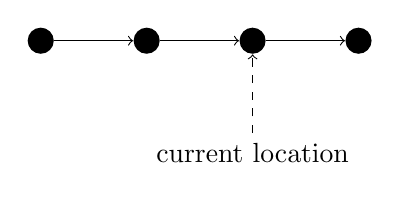
\begin{tikzpicture}[start chain,every join/.style={->}]
            \draw
                node[history] {}
                node[history] {}
                node[history] (here) {}
                node[history] {}
                ;
            \draw[->,dashed]
                node[below=of here] (pt) {current location}
                (pt) -- (here)
                ;
        \end{tikzpicture}
    \end{center}
    \caption{A simple linear edit history}
    \label{fig:linear history}
\end{figure}

There are at least two orthogonal directions this baseline can be improved.
First, the history itself can be given additional structure: rather than
discarding the ``redo future'' whenever making a change, the model could
simply branch, resulting in a richer edit history than a straight line --
perhaps a tree or even a DAG. (Figure~\ref{fig:branching history} gives an
example of this.) It then becomes natural to ask whether changes from one
branch can be migrated to another branch. Many papers examine this
question~\cite{abowd1992giving,berlage1994selective,cass2007using,dix95moving,kurlander1990visual};
one of the major lessons is that representing edits with rich data about the
\emph{intention} of the user makes the algorithms much more predictable and
usable.

\begin{figure}
    \begin{center}
        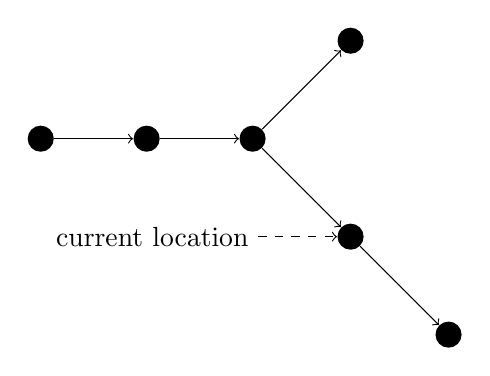
\begin{tikzpicture}[start chain=beginning,every join/.style={->}]
            \draw
                node[history] {}
                node[history] {}
                node[history] {}
                ;
            \begin{scope}[start branch=upper going above right]
                \draw
                    node[history] {}
                    ;
            \end{scope}
            \begin{scope}[start branch=upper going below right]
                \draw
                    node[history] (here) {}
                    node[history] {}
                    ;
            \end{scope}
            \draw[->,dashed]
                node[left=of here] (pt) {current location}
                (pt) -- (here)
                ;
        \end{tikzpicture}
    \end{center}
    \caption{A more complex edit history}
    \label{fig:branching history}
\end{figure}

Thus, a second possible axis of improvement, which we will focus on in this
paper, is modifying the edits to operate on parse trees rather than simple
character sequences. Note that the requirements for these tree edits are
somewhat different from the requirements cited for revision control systems:
\begin{itemize}
    \item Rolling back ill-advised changes
    \item Visualizing changes in a human-readable way
    \item Relocating changes within the history meaningfully
\end{itemize}
In particular, computing edits given two trees is no longer a key feature;
the editor itself can track the \emph{actual} edits made by the user.
Tracking provenance is likewise unneeded.

The final application area we will consider is that of an XML-backed
database, backing, say, a web application. The edits, therefore, are in fact
a form of communication between the web application and the database, rather
than being manipulated in memory (or on disk) from within a single program,
as in revision control systems or text editors. Moreover, the bulk of the
edit will be hand-composed by a human (namely, the programmer developing the
web application) -- though it may have some holes or variables to be filled
in at run time. For our purposes, we may well assume that an edit will be
executed much, much more frequently than it is composed.

As a result, the requirements of an edit language for databases are
radically different than those for revision control systems or text editors.
In particular, a web application often has multiple users, and consequently
may submit many edits to the database simultaneously; the database should
behave as though they were submitted in some order (though it may execute
them concurrently). Combining these characteristics, we find that doing some
one-time analysis of edits can be very worthwhile if the results of the
analysis can be used to speed up the application of those edits at runtime,
because the benefits of the analysis will be reaped many times, but the cost
paid only once. So a successful edit language should have these properties:
\begin{itemize}
    \item Human-writable, text-based syntax
    \item Compact representation for inter-program communication
    \item Speedy concurrent apply operation (perhaps via a helpful static
        analysis)
\end{itemize}
(Note that in particular this application may not place such high priority
on the ability to roll back changes.)
\end{newcontent}

There is unending variety in edit languages. Indeed, even when considering
the data objects that the edits are intended to modify, there are a huge
number of different models possible: binary (opaque) data, sequences,
sets, trees, relations, DAGs, graphs, and more. Each of these could
presumably have a whole collection of reasonable choices of edits from
simple to expressive. On one end of the spectrum, we have the diff format
for editing sequences; on the other end lies programs written in (say) C
that edit any data type we could imagine; somewhere in the middle lie
relations and the relational calculus. Surveying all the known edit
languages is well beyond the scope of this paper. Instead, we will consider
only node-labeled, unordered trees as our data model, and consider just a
few languages that cover a range of the expressiveness spectrum.

We will also narrow our focus to only three edit languages. The L\"oh, et al
paper strives to introduce a framework for reasoning about the behavior of
revision control systems~\cite{loh2007principled}. It will include more
precise definitions for words we have so far been using informally: edits,
edit history, conflict and compatibility, merging, synchronization, and so
forth. The second language (as described in the Chawathe and Garcia-Molina
paper~\cite{chawathe1997meaningful}) is designed to include an expressive
enough core that machine-generated edits can encapsulate the ``idea'' or
``meaning'' of a change while keeping tractable computation of a (nearly)
minimal diff between old and new trees.  Finally, the third language
(introduced in the Ghelli, et al paper~\cite{ghelli2006commutativity}) is
designed to make deciding whether two edits depend on each other---to be
more precise, whether they commute---tractable, while emphasizing the
inclusion of high-level features designed to make the language
human-writable.

Before diving in, we briefly describe a few typographic and metasyntactic
conventions. Variables $d$ and $e$ will correspond to concrete pieces of
data and edits, respectively. Edits will have a partial function \apply
associated with them; $\apply(e,d) = d'$ indicates that edit $e$ transforms
data $d$ to data $d'$, and $\apply(e,d) = \undefined$ indicates that edit
$e$ is incompatible with data $d$. The definition of \apply will vary
between sections.  Additionally, we will assume an infinite supply $L$ of
labels; we will use metavariable $\ell$ for an element of this set. We will
use $\symdiff$ for the symmetric difference and $\#$ for set disjointness.

\section{Semantics and conflict detection}
\label{sec:semantics}
We will begin our discussion by developing a formal framework in which we
can define precisely terms like \emph{edit history}, \emph{edit},
\emph{working copy}, \emph{merge}, and \emph{conflict}. (We will also
sometimes use \emph{repository} interchangeably with edit history, and
\emph{patch} interchangeably with edit.) The aim of the current exercise is
to develop a semantic model we can use to unify a variety of edit languages,
following the development of L\"oh, et al~\cite{loh2007principled}.

\subsection{Data and edits}

As mentioned above, we will use node-labeled trees as our data model; in
fact, we will demand that node labels have two parts: a \emph{name} drawn
from $L$ and some \emph{contents} drawn from another arbitrary set $C$. (For
example, when this is modeling a file system, $L$ would be the set of valid
filenames, and $C$ would include information like permissions and the bytes
in the file.) Moreover, we will use a somewhat idiosyncratic representation
of these trees; we will defend the idiosyncrasies in
Section~\ref{sec:flexibility}.

For our purposes, a tree is a set of assertions $A$, where each $a \in A$
has the form
\begin{align*}
    a &::= \ell_p \to \ell_c \mid \ell \contains c \\
    c &::= \mbox{(elements of C)},
\end{align*}
and where $A$ conforms to the well-formedness constraints given in
Figure~\ref{fig:well formed tree}. We assume the existence of a
distinguished label $\root \in L$, and adopt the convention that variables
free in the premise of an inference rule are bound universally, while
variables free in the conclusion (that are not bound in the premise) are
bound existentially. Rule \rn{Parent} says that each node has at most one
parent. The \rn{UniqC} rule tells us that each node is labeled with at
most one piece of content. Rules \rn{Full1}, \rn{Full2}, and \rn{Reachable}
together say that every node is labeled and reachable from \root. Finally,
rule \rn{Cycle} rules out cycles.

\begin{figure}
    \infrule[Parent]
        {\ell_p \to \ell_c \\ \ell_p' \to \ell_c}
        {\ell_p = \ell_p'}
    \vspace{2ex}
    \infrule[UniqC]
        {\ell \contains c \\ \ell \contains c'}
        {c = c'}
    \vspace{2ex}
    \infrule[Full1]{}{\root \contains c}
    \vspace{2ex}
    \infrule[Full2]{\ell \to \ell'}{\ell' \contains c}
    \vspace{2ex}
    \infrule[Reachable]
        {\ell \contains c}
        {\root = \ell_0 \land (\forall i \in
        \{0,\ldots,n\}. \ell_i \to
        \ell_{i+1}) \land \ell_n = \ell}
    \vspace{2ex}
    \infrule[Cycle]
        {\forall i \in \{0,\ldots,n\}.\ell_i \to \ell_{i+1}}
        {\ell_0 \ne \ell_n}
    \caption{Invariants that guarantee tree-structure}
    \label{fig:well formed tree}
\end{figure}

At its core, an edit to this structure is simply an object $(S,T)$ with
a set of assertions $S$ to remove and a set of assertions $T$ to add. We
could then say that the patch is applicable to $d$ when $S \subset d$, that
is, when all of the assertions that the patch aims to remove are available.

However, this proposal has a small flaw: it makes no mention of the
invariants of $d$. Indeed, there are certain kinds of patches which, no
matter how we construct them, cannot guarantee that it maintains the
invariants whenever it is applicable. Consider, for example, the edit that
simply inserts a new top-level node at $\ell$ with contents $c$, namely
$(\emptyset,\{\ell \contains c,\root \to \ell\})$. In most trees, this is
fine, but if the top-level node $\ell$ already exists with contents other
than $c$, then applying this patch would break \rn{UniqC}. Thus, we would
like a way to say that certain assertions do not exist in the data, namely,
any assertion assigning contents to $\ell$.

We can solve this problem by adding a third element to the definition of a
patch: a set of forbidden assertions. We thus arrive at our final
definitions for patch and applicability:

\begin{definition}
    A \emph{patch} or \emph{edit} is a triple $(S,E,T)$ where $S \cup T
    \subset E$.
\end{definition}
We will sometimes write $(S,\_,T)$ when we mean $(S,S \cup T,T)$.
\begin{definition}
    An edit $(S,E,T)$ is \emph{applicable} to data $d$ when $E \cap d = S$,
    and
    \[\apply((S,E,T),d) = \left\{\begin{tabular}{cl}
        $d \symdiff S \symdiff T$   & $(S,E,T)$ is applicable to $d$ \\
        \undefined                  & otherwise
    \end{tabular}\right..\]
\end{definition}

(It is worth pointing out that $E \cap d = S$ implies, in particular, that
$S \subset d$.)

Revisiting the example above, we can now write
\[e_1 = (\emptyset,\{\root \to \ell\}\cup\{\ell \contains c' | c' \in
C\},\{\root \to \ell, \ell \contains c\})\]
for the patch that adds a new top-level node. Unlike the previous proposal,
we can now state with confidence that whenever $e_1$ is applicable to $d$,
the application $\apply(e_1,d)$ will preserve the invariants of our tree
structure. Of course, we can still write patches that will violate the
invariants; however, what we can do with this definition of a patch that we
could not do with the first proposal is we can write patches for which we
can prove that they will never violate the invariants when they are
applicable.

For convenience, we will adopt the following abbreviation.  When the
iteration domain is clear from context, we will write $*$ as a placeholder
for all values in that domain; so $\{\ell \contains c' | c' \in C\}$ could
be shortened to $\{\ell \contains *\}$, for example. Each appearance of $*$
is independent. Using this notation, the above patch would look like this:
\[e_1 = (\emptyset,\{\root \to \ell,\ell \contains *\},\{\root \to \ell,\ell
\contains c\})\]

As another example patch, consider adding a node lower in the tree, as a
child $\ell_c$ with contents $c_c$ of $\ell_p$ (which has contents $c_p$).
To preserve the invariants, we must make sure not only that there is no node
already at $\ell_c$, but also that the parent node $\ell_p$ exists.  We can
achieve this by putting $\ell_p \contains c_p$ in both $S$ and $T$, that is,
by requiring $\ell_p \contains c_p$ to be in the data before application,
and to include it after application.
\begin{align*}
    S_2 &= \{\ell_p \contains c_p\} \\
    E_2 &= \{\ell_p \contains c_p, * \to \ell_c, \ell_c \contains *\} \\
    T_2 &= \{\ell_p \contains c_p, \ell_p \to \ell_c, \ell_c \contains c\} \\
    e_2 &= (S_2,E_2,T_2)
\end{align*}

\subsection{Constructors for common patches}
With this framework in place, we can define some syntax for common tree
operations. None of the theory in the following parts depend directly on the
existence of this syntax or their interpretations, but they serve as a good
way of illustrating the concepts introduced so far.  We will define syntax
for four operations: node insertion, updating the contents of a node,
reparenting or moving a subtree, and copying a subtree.

For insertion, we will allow the inserted node to ``steal'' some of its
siblings to use as children. That is, we will specify a label and contents
for the new node, a parent for the new node, and a collection of the parent
node's children that should become children of the new node. We will also
restrict the nodes that we insert to ones not already in the tree. Thus:
\begin{align*}
    \einsert(\ell_p,\ell_c,c_c,L_c) ={}
        & (\{\ell_p \to \ell \mid \ell \in L_c\}, \\
        & \{\ell_p \to \ell \mid \ell \in L_c\} \cup
          \{\ell_c \to \ell \mid \ell \in L_c\} \cup
          \{* \to \ell_c, \ell_c \contains c_c\}, \\
        & \{\ell_p \to \ell_c,\ell_c \contains c_c\}\cup\{\ell_c \to \ell
        \mid \ell \in L_c\})
\end{align*}

Updating the contents of a node and moving subtrees are perhaps the easiest
of the patches to represent in our framework:
\begin{align*}
    \eupdate(\ell,c_{\mathit{old}},c_{\mathit{new}})
        &= (\{\ell \contains c_{\mathit{old}}\},\_,\{\ell \contains
        c_{\mathit{new}}\}) \\
    \emove(\ell_c,\ell_p,\ell_p')
        &= (\{\ell_p \to \ell_c\},\_,\{\ell_p' \to \ell_c\})
\end{align*}

Copying a subtree is a bit more involved. We must first identify a subtree;
let us say that $S$ is a set of assertions that satisfy the invariants given
above (but with a different distinguished \root; call it $\root_S$). To copy
this subtree, we must choose new node labels. Suppose $f:L \to L$ is a
relabeling function. Lift $f$ to an assertion relabeling function:
\begin{align*}
    f(\ell \contains c) &= f(\ell) \contains c \\
    f(\ell \to \ell') &= f(\ell) \to f(\ell')
\end{align*}
Lift $f$ to sets of labels and sets of assertions in the natural way. We
will also say that $\ell\mbox{ in }S$ when $\ell \to \ell' \in S$ or $\ell'
\to \ell \in S$ or $\ell \contains c \in S$. Then we can define
\begin{align*}
    \ecopy(S,\ell,f) ={}
        & (S, \\
        & S \cup f(S) \cup \{* \to \ell_c | \ell_c\mbox{ in }f(S)\}, \\
        & f(S) \cup \{\ell \to f(\root_S)\})
\end{align*}
for injective $f$.  The additional constraint $\{* \to \ell_c | \ell_c\mbox{
in }f(S)\}$ ensures that all of the labels generated by $f$ are actually new
for the tree.

As a bonus, patches inverse gives us a node deletion operation for free (by
inverting \einsert), as well as a slightly weirder \emph{glue} operation
(from inverting \ecopy) which merges two identical subtrees, causing one to
disappear.

\subsection{A comment on flexibility}
\label{sec:flexibility}
It is worth taking a moment to address the question that is no doubt on the
reader's mind: why are we using such a weird representation of trees?

We could certainly have stated all of the definitions given so far in a more
familiar way: we could represent trees in the usual way as a collection of
nodes and edges, with a labeling function mapping node identifiers to their
contents.  The definition of what a patch is would have to be modified, as
well, to include more specific notions of nodes and edges, ways of modifying
the labeling function, and allow for more tree-specific preconditions. (For
example, we might choose analogs to the syntax given above as the primitive
edits, or some variant of them.)

The result, however, would have the definition of patch hopelessly
interwoven with the particular kind of data that patch is modifying. The
presentation here has the much nicer property of being data-agnostic when
defining the meaning and applicability of patches. As a result, the
definitions above (and the definitions below) can be used verbatim even if
the data model changes: the ideas here apply equally well to different data
structures.

Of course, some things change. For different data structures, we must choose
a different collection of basic assertions, and rework the invariant that
the whole collection of assertions must satisfy. However, these extensions
are generally quite self-contained.

\subsection{Repositories and edit histories}
The least well-understood ideas in revision-control system are those of
merging and conflicts. To work towards understanding these ideas, we now
attempt to define properly what a repository is and how repositories can
interact.

\begin{definition}
    A \emph{working copy} is a tree (represented as described above).
\end{definition}
\begin{definition}
    A \emph{repository} is a bag of patches.
\end{definition}

These definitions are deceptively simple. For example, the simplest question
we might ask is, ``How are repositories and working copies related?''. We
can build up a working copy by applying a sequence of patches to the empty
set of assertions. However, given only a repository, we are at something of
an impasse: the patches are unordered, and we are not at all guaranteed that
if we choose an arbitrary order that application will be well-defined, or
even that any ordering exists that makes application well-defined. We will
therefore call a repository \emph{consistent} when there is an ordering of
the patches $\left<e_0,\ldots,e_n\right>$ such that, given $d_0 =
\emptyset$, each $d_{i+1} = \apply(e_i,d_i)$ is well-defined, that is,
$d_{i+1} \ne \undefined$. It is convenient that if two such orderings exist,
they result in the same final working copy (thanks to the commutativity of
$\symdiff$).

With that concept in hand, we can define merges and conflicts.

\begin{definition}
    Given two consistent repositories $R_1$ and $R_2$ and a set of patches
    $P \subset R_2 \setminus R_1$ that we would like to transport from $R_2$
    to $R_1$, we say that $R_1 \cup P$ is successfully \emph{merged} when
    $R_1 \cup P$ is consistent, and that it is in \emph{conflict} otherwise.
\end{definition}

% TODO: example of a conflict, plus how to deal with it (expanding $P$ or
% human intervention)

\subsection{Discussion}
We now have a firm definition for many of the ideas we will discuss in this
paper. The definitions are concise; they are elegant in their coverage and
orthogonality. However, there are a few significant shortcomings of the
development so far.

The first is that a direct translation of these ideas to code would be
impractical. Many of the common patches discussed above involve manipulating
infinite sets, which makes the problem a non-starter. Of course, this can be
combated in most cases by judicious choice of the representation of a patch.
For example, some algebraic data structure involving the patch constructors
above, patch composition, and patch inverse might be reasonable. The role of
the work discussed here, then, is to provide a model against which to verify
the manipulations of these higher-level representations. Similarly, a real
implementation would need a similar process for designing a more concrete
representation of repositories and working copies, appealing to the simple
set-based model when verifying algorithm correctness.

A second serious drawback is the simplicity of the working copy that we
used. However, this drawback is not inherent to the approach. Indeed, the
exposition by L\"oh, et al demonstrate extensions to the model that allow
for line-based files, repository meta-data, and tagging. Some similar
extensions are likely possible for tracking patch ordering information, if
that becomes desirable.

Finally, we have so far seen only very idealized definitions, and no
practical algorithms. For example, we have not discussed any practical way
of checking even the consistency of a given repository! In practice, we
would also want algorithms for computing minimal patch sets that
successfully merge and for comparing two working copies. These may be quite
difficult in practice.

\begin{newcontent}
We can revisit the criterion discussed in Section~\ref{sec:introduction} for
revision control systems, text editors, and databases to evaluate how far
this approach takes us.

One feature we want in revision control systems is the ability to roll back
ill-advised changes. The current approach actually gives us \emph{two} ways
of doing this. The first is to add an inverse patch\footnote{The inverse of
$(S,E,T)$ is $(T,E,S)$, of course.} to the repository; this records that we
made an edit and later decided it was a bad idea. The second is to remove
the patch from the repository entirely; we can do this if we want to pretend
that we never did that edit in the first place. So that criteria seems
well-covered.

We would also like an algorithm for detecting changes; the current approach
does not provide such a thing, but the approach of the next section attempts
to handle this. For reconciling changes made in parallel, the current
approach seems to give us a good definition of what it would mean to do this
(that is, a successful merge reconciles different repositories), but gives
no hint of how to implement a tractable merge algorithm. (This does not seem
to be a fundamental limitation of the approach -- but simply something that
has not \emph{yet} been solved.) Finally, the problem of tracking provenance
is tackled somewhat in the paper (though the details have been omitted here
for space).

For text editors, in addition to rollback, we also want visualizations and
change relocation. While a good visualization is likely possible, none of
the discussion so far has focused on it; getting this right would likely
take some serious work. On the other hand, relocating changes within the
history is almost trivial in this framework. Since a repository is an
unordered set of patches, relocating a patch is the identity!

So this approach is a mild success for revision control and text
editing; but it seems to fail all three criteria for a database system.
Patches of this form are not particularly human-writable; as mentioned
above, some serious thought would be required even to represent these
patches in memory; and finally, there is no clear provision for concurrency.
We will need another approach for databases.
\end{newcontent}

\section{Change detection}
\label{sec:detection}
\subsection{Problem description}
In this section, we will develop one of the missing algorithms, following
the development of Chawathe and Garcia-Molina~\cite{chawathe1997meaningful}.
The problem statement is fairly simple: we have two working copies (say, one
from a repository and one from the disk), and we would like to generate a
patch to convert one working copy to the other.

Actually, the problem as stated is quite simple: given working copies $S$
and $T$, the patch $(S,\_,T)$ satisfies the criteria. It is nevertheless
clearly not the desired patch. To narrow the problem, we introduce a cost
function for patches; we then wish to find not just any patch, but a
minimal-cost patch. We will allow sequences of patches of the simple forms
introduced in the previous section\footnote{We can \apply a patch sequence
by using \apply on the composition of the patches in the sequence. Deriving
the triple for the composition of two patches is easy, but tangential.}.

Dozens of variants of this problem have been
studied~\cite{chawathe1997expressive,chawathe1996change,cobena2002detecting,wang2004x}.
Points of variation include:
\begin{itemize}
    \item The exact details of how each edit behaves often differ, though
        they are usually fundamentally similar to the ones proposed above.
    \item Different approaches consider cost functions of varying
        sophistication.
    \item Some analyses assume that nodes have identities which can be
        compared between working copies, and others do not make this
        assumption.
\end{itemize}
One of the major interactions between the first two variations involves how
the cost function behaves on moves and copies. Some analyses simply disallow
moves and copies (which is tantamount to simply making them prohibitively
expensive compared to deleting and inserting nodes). These analyses benefit
from much greater simplicity; however, the edits generated by them can be
somewhat surprising to human readers. On the other hand, making moves and
copies cheap enough that they must be considered during the analysis
elevates the problem to NP-hardness.

For now, we will make the following decisions:
\begin{itemize}
    \item As mentioned above, we will use exactly the edits described in
        Section~\ref{sec:semantics}.
    \item We will use a fairly simple cost function: we will have constants
        $c_i$, $c_d$, $c_m$, $c_c$, and $c_g$ for the costs of \einsert,
        inverse \einsert (i.e. deletion), \emove, \ecopy, and inverse \ecopy
        (i.e. glue), respectively. For the cost of an \eupdate, we will
        allow an arbitrary function $c_u:C \times C \to \mathbb{R}$ to give
        the cost given old and new contents.
    \item We will not assume that nodes have persistent identities; the
        detection algorithm will have to discover correspondences on its
        own.
\end{itemize}
In particular, the costs of \emove and \ecopy will likely be quite low
compared to moving and copying entire subtrees. To avoid exponential running
time, the algorithm presented will have to make approximations in a few
places; we will point them out as they arise.

The solution we present has two main pieces: first, finding an
\emph{alignment} or correspondence between the nodes of the two working
copies, and then converting that alignment into a low-cost edit.

\subsection{Alignment discovery}
Define the operator $(-)^+$ to add a fresh, newly-labeled, disconnected node
to a tree. (The contents of the node are immaterial for our purposes.)
Below, we will assume the freshly chosen label is $+$.

\begin{definition}
    An \emph{alignment} between $d_1$ and $d_2$ is a minimal edge cover of
    the complete (unweighted) bipartite graph whose parts are the node
    labels of $d_1^+$ and the node labels of $d_2^+$.
\end{definition}

Recall that an edge cover of a graph is a subgraph with all the nodes and in
which each node has degree at least one. A minimal edge cover is one which
achieves this with the minimal number of edges (for unweighted graphs) or at
minimal cost (for weighted graphs). Thus, an alignment gives a
correspondence between the nodes of the two graphs via its edges: if there
is an edge $(a,b)$ in the alignment, we read this as meaning that the
edit we compose should turn node $a$ in $d_1$ into node $b$ in $d_2$.
Similarly, an edge $(a,+)$ indicates that the edit we compose should delete
$a$ from $d_1$, and an edge $(+,b)$ indicates that the edit should create
$b$ from scratch.

% TODO: perhaps include a picture here
% For example, consider the straw-man edit we suggested in the overview.
% That edit deleted all of the nodes in $d_1$, then inserted all of the
% nodes in $d_2$. This could be represented in an alignment like this:
% \begin{tikzpicture}
%     nodes and children and edges, oh my!
% \end{tikzpicture}

We will assign to each alignment the cost of the patch that results from
that alignment, and our goal will be to find a minimal alignment. We must
therefore turn to the problem of converting an alignment into a patch. What
we will hope to do is to assign a weight to each edge of the complete
bipartite graph in such a way that choosing a minimal cover of the
\emph{weighted} graph corresponds to choosing a minimal alignment.

\subsection{Converting from alignment to edit}
One algorithm involves simply converting each edge in the alignment to a few
atomic updates, as well as some global ordering constraints on which edges'
updates should come earliest. It proceeds by case analysis on the edge:
\begin{itemize}
    \item $(+,+)$: No edit is needed for this edge.
    \item $(a,+)$: Check which other nodes have edges to $+$. If $c_g<c_d$,
        that is, inverse \ecopy is cheaper than inverse \einsert, then look
        for another node with the same label which we can glue to. If so,
        generate an inverse \ecopy, possibly prefixed by an \eupdate, and
        a constraint saying that the deletion of the other node must come
        after these edits. If no suitable glue operation exists, generate a
        deletion.
    \item $(+,b)$: Similarly to the previous case, check which other nodes
        have edges from $+$. If $c_c<c_i$, that is, \ecopy is cheaper than
        \einsert, then look for another node with the same label that we can
        copy. If so, generate a \ecopy, possibly followed by an \eupdate,
        and a constraint saying that these must come after the creation of
        the node we are copying.  If no suitable copy operation exists,
        generate an \einsert.
    \item $(a,b)$: By far the most complicated of the bunch. Naively,
        this would be a \emove or a \ecopy possibly followed by an \eupdate.
        However, we should first walk up the tree, so that we \emove or
        \ecopy the highest possible node; that node's subtrees will then get
        moved or copied ``for free''.

        In fact, there is an additional wrinkle. Suppose there is a \ecopy
        operation high in the tree, and another operation \emove{}s a
        node somewhere in the subtree that is being copied. We may now
        choose whether the copy that we create includes or does not include
        that node by choosing to perform the \emove before or after the
        \ecopy. Thus, the algorithm must also include some logic which
        evaluates such situations (called ``free copies'' in the Chawathe,
        et al exposition) to minimize the number of \emove and \ecopy
        operations; we will skip the details of this logic.

        % TODO: a picture would be really good here, too
\end{itemize}
After this algorithm runs, the edges are topographically sorted (using the
constraints generated as the topography), and the atomic edits are sequenced
in the resulting order.

% TODO: consider giving an example where update order matters -- i.e. where
% we get a free copy or something like that

The algorithm itself may sound somewhat complicated, but the take-away
message is fairly simple: there is no such thing as the ``cost of an edge''
in the complete bipartite graph. The cost of the updates generated by any
particular edge in this graph depends on what other edges exist in the
particular alignment chosen. As a result, we cannot simply give weights to
the edges of the complete bipartite graph as we had hoped.

The development by Chawathe and Garcia-Molina adopts a slightly more subtle
approach: each edge is given an upper and lower bound on the cost that could
be incurred by including a particular edge. It is then possible to prune
away obviously bad edges; as the complete graph is reduced, the bounds are
improved, making more pruning possible. We will skip the algorithms involved
in computing the initial bounds, pruning bad edges, and updating the bounds
as the graph evolves; they are clever, but not central to the idea.

When this process terminates, we have a small, bipartite graph, where each
edge is labeled with upper and lower bounds. We can use the lower bounds as
estimates of the cost each edge contributes to the alignment and run a
standard weighted matching algorithm to find an approximately minimal cover.
Given this cover, we can then generate the edit corresponding to the cover,
as described above.

\subsection{Discussion}
Before addressing the strengths and weaknesses of this approach, we pause to
explicitly identify the places in the algorithm where approximations are
made (leading to occasionally sub-optimal edits). First, the final edit we
create is generated from an alignment, and our algorithm for converting
alignments into edits is not surjective. For example, any single node in the
tree gets assigned at most one of the \einsert, inverse \einsert, \emove,
\ecopy, or inverse \ecopy edits and at most one \eupdate edit. Furthermore,
the generated edit will never modify nodes that are in neither tree -- for
example, by creating a new node, doing something with it, and then deleting
it. Finally, no generated edit will perform an inverse \ecopy on any node
involved in a normal \ecopy, either directly or indirectly. Each of these
restrictions may seem spurious, but in fact violating them can be useful;
thus, failing to generate edits that violate them is approximation number
one.  Still, whether this approximation is good or bad is somewhat
philosophical; the edits that take advantage of the extra abilities outlined
above are often somewhat tricky, and may be surprising to a human reader.

The second approximation comes at the end, when choosing a minimal cover in
the weighted bipartite graph. Since there is no true weight for the edges in
the graphs, the labeling chosen (for example, using the lower bounds) must
be an approximation. In some cases, there may be few enough possible covers
that we can perform an exhaustive search, but often this will not be the
case. Luckily, this is an approximation with a knob that we can twiddle: we
can improve our edits (at the cost of runtime) by examining more possible
covers and choosing the minimal one out of the ones we examine.

The algorithm outlined above is admittedly quite complex. Because of the two
approximations mentioned, it is also somewhat heuristic -- there are no
theoretical guarantees about its output, and so it could potentially have
somewhat unpredictable behavior. Additionally, the complexity makes this
approach somewhat inflexible to variations in the set of edits. The
conversion between alignments and minimal edits as well as the cost
estimation algorithms are fairly dependent on using exactly the set of edits
described above.

Despite these shortcomings, this approach also has several nice properties.
It is fairly fast; for $n$ nodes, it is $O(n^3)$ worst-case, and
experimentation suggests that it is $O(n^2)$ for the typical case. The cost
model proposed is fairly flexible, as well. Moreover, detecting node moves
and copies is a nice feature.
\begin{newcontent}%
For example, in the revision control system domain, detecting moved or
copied files is key for maintaining provenance information. Many current
systems either require the user to manually specify moves and copies or
apply some easily-fooled ad-hoc heuristics for detecting them. Reliably
analyzing this kind of code motion could be very beneficial for these
systems.

Thus, this approach remedies one of the shortcomings of the previous
approach for use in a revision control system. Additionally, it makes some
small strides in the text-editor and database domain by providing a compact,
concrete representation for edits. It is possible that either the alignments
discussed above or the actual edit sequences computed could be readily
visualized by a human; similarly, it seems much more feasible for a human to
construct one of these edits and for programs to exchange these edits than
than it was for edits of the form discussed in Section~\ref{sec:semantics}.
Still, it leaves much to be desired for human-writability; we will need to
consider another approach for our edits to be sufficiently high-level.
\end{newcontent}

\section{Reordering}
\label{sec:commutativity}
In the previous section, we discussed an edit language designed primarily
for machine generation, with a passing interest in human readability. As a
result, we ended up with a language that had a few very low-level editing
capabilities, and the only way of creating large-scale edits was by chaining
together many, many small-scale edits. In this section, we will instead
focus on a language designed for human generation. It will feature
high-level abstraction mechanisms for iteration and scoping, allowing for
concise descriptions of large-scale edits. As a trade-off, the kind of
analysis described for finding minimal edits achieving a certain effect will
likely be impossible or intractable; nevertheless, another kind of analysis
for detecting whether two edits are sensitive to application order is still
possible.

This language was designed from the perspective of database maintenance.
There are a great variety of such languages, including myriad variants of
SQL (based on the relational calculus~\cite{codd1970relational}), Datalog
(for querying deductive databases~\cite{minker1987foundations}),
XQuery~\cite{boag2002xquery} (for querying XML databases) and variants that
include updates~\cite{sur2004xquery}, LINQ~\cite{meijer2006linq} (which
strives in part to unify several database implementations), and so on. Our
focus on tree-based data makes XML the most natural representation choice
out of these; correspondingly, the language we describe below will be
inspired by XQuery.

Properly describing the behavior of the high-level edit language described
in the Ghelli, et al paper~\cite{ghelli2006commutativity} involves first
defining a low-level edit language much like the one described in the
previous section, so we will begin there -- in familiar territory.

\subsection{Edit history}
The data model we consider here is slightly more intricate than before.  We
assume some primitive form of locations \loc that can express at least URIs
and positions in code, a set of names $Q$, and a set of possible text
content elements $T$. Assertions look like this:
\begin{align*}
    a ::={}
    & \exists\ell \mid \ell\to\ell' \mid \ell\isfrom\loc \mid \\
    & \ell \has K \mid \ell \named Q \mid \ell \contains T \\
    K ::={} & \ktext \mid \kelement
\end{align*}

The invariants are listed in Figures~\ref{fig:routine store}
and~\ref{fig:interesting store}. The invariants in
Figure~\ref{fig:routine store} essentially enforce tree-structure (though it
allows for subtrees that are not actually connected to anything, which we
will use later during deletion). We can view the set of assertions of the
form $\exists\ell$ as being a set of nodes. Then rules \rn{DomLoc},
\rn{DomName}, and \rn{DomKind} say that\isfrom assertions,\named assertions,
and\has assertions only apply to nodes that we know about. Together with
rules \rn{FuncLoc}, \rn{FuncName}, and \rn{FuncKind}, this implies that the
assertions are actually partial functions whose domain is the set of nodes.
Rule \rn{TotKind} further tells us that the\has assertions actually
represent a total function. Rules \rn{Parent} and \rn{Cycle} are identical
to the previous sections, and say simply that each node has at most one
parent and that there are no cycles.

\begin{figure}
    \infrule[DomLoc]{\ell\isfrom\loc}{\exists\ell}
    \vspace{2ex}
    \infrule[DomName]{\ell \named q}{\exists\ell}
    \vspace{2ex}
    \infrule[DomKind]{\ell \has k}{\exists\ell}
    \vspace{2ex}
    \infrule[FuncLoc]
        {\ell\isfrom\loc \andalso \ell\isfrom\loc'}
        {\loc = \loc'}
    \vspace{2ex}
    \infrule[FuncName]
        {\ell \named q \andalso \ell \named q'}
        {q = q'}
    \vspace{2ex}
    \infrule[FuncKind]
        {\ell \has k \andalso \ell \has k'}
        {k = k'}
    \vspace{2ex}
    \infrule[TotKind]{\exists\ell}{\ell \has k}
    \vspace{2ex}
    \infrule[Parent]
        {\ell_p \to \ell_c \andalso \ell_p' \to \ell_c}
        {\ell_p = \ell_p'}
    \vspace{2ex}
    \infrule[Cycle]
        {\forall i \in \{0,\ldots,n\}.\ell_i \to \ell_{i+1}}
        {\ell_0 \ne \ell_n}
    \caption{Routine invariants for XML-like trees}
    \label{fig:routine store}
\end{figure}

The invariants in Figure~\ref{fig:interesting store} are slightly more
interesting. Rule \rn{LocRoot} says that only root nodes have source
location. Rules \rn{ElemNamed1} and \rn{ElemNamed2} together say that nodes
have a name iff they are element nodes; similarly, \rn{TextFull1} and
\rn{TextFull2} together say that nodes have textual content iff they are
text nodes. Finally, rule \rn{TextLeaf} only allows leaf nodes to be text
nodes (that is, text nodes have no children).

\begin{figure}
    \infrule[LocRoot]{\ell\isfrom\loc}{\forall \ell'.\lnot(\ell' \to \ell)}
    \vspace{2ex}
    \infrule[ElemNamed1]{\ell \has \kelement}{\ell \named q}
    \vspace{2ex}
    \infrule[ElemNamed2]{\ell \named q}{\ell \has \kelement}
    \vspace{2ex}
    \infrule[TextFull1]{\ell \has \ktext}{\ell \contains t}
    \vspace{2ex}
    \infrule[TextFull2]{\ell \contains t}{\ell \has \ktext}
    \vspace{2ex}
    \infrule[TextLeaf]{\ell \to \ell'}{\ell \has \kelement}
    \caption{Interesting invariants of XML-like trees}
    \label{fig:interesting store}
\end{figure}

From here, we will define a few atomic updates in the edit-triple form
described in Section~\ref{sec:semantics}. (When there may be some confusion,
we will refer to these as atomic edits or low-level edits.  We will refer to
expressions in the later edit language as high-level edits.) When $A$ is a
well-formed set of assertions that does not contain any assertions of the
form $\ell\to\ell'$ or $\ell \isfrom \loc$ -- that is, when $A$ contains a
set of new nodes to add, possibly with text content or names, but no edges
or locations -- we will allow them to be created:
\begin{align*}
    \einsert_n(A) &= (\emptyset,\_,A)
\end{align*}

Given a node and a location, we can extend the location mapping. The middle
precondition ensures that we only give locations to root nodes.
\begin{align*}
    \einsert_r(\ell,\loc) ={}
        & (\{\exists\ell\}, \\
        & \{\exists\ell,*\to\ell,\ell\isfrom*\}, \\
        & \{\exists\ell,\ell\isfrom\loc\})
\end{align*}

Given a set of assertions $E$ of the form $\ell_p\to\ell_c$, we can add
those edges to the working copy. Below, we will use the set
$N=\{\exists\ell_p,\exists\ell_c | \ell_p\to\ell_c \in E\}$ of nodes
involved. We will also arrange for the addition of $E$ to avoid creating
cycles (though we do not represent this fact in the definition of the edit).
\begin{align*}
    \einsert_e(E) ={}
        & (N, \\
        & N\cup\{*\to\ell_c,\ell_c\named* | \ell_p\to\ell_c \in E\}, \\
        & N \cup E)
\end{align*}

Finally, we allow the deletion of edges. Nodes may be deleted, but only by
disconnecting their subtree from the top-level tree of interest -- that is,
by deleting the edge from their parent -- never by removing them from the
working copy. So, letting $E$ be a set of assertions of the form
$\ell_p\to\ell_c$ and using the $N$ abbreviation as before, we have
\[\edelete_e(E) = (E \cup N,\_,N)\]
When we are writing an edit for a particular piece of data $d$, we will
adopt the notation $\edelete_e(S)$ to extract all the edges pointing to
nodes in $S$ from the data and delete them, that is,
\[\edelete_e(S) = \edelete_e(\{\ell_p \to \ell_c \in d \mid \exists\ell_c
\in S\})\]

Later, the programs we write in the high-level language will be run on a
particular working copy to produce a sequence of these low-level edits, and
it will be this pairing of a working copy and edit sequence that we are
interested in analyzing.

\begin{definition}
    A \emph{store history} $\eta$ is a pair $(d,\bar e)$, where $\bar e$ is
    a sequence of edits $\left<e_1,\ldots,e_n\right>$ to be \apply'd in
    turn.
\end{definition}

We will occasionally abuse notation, and write $f(\eta)$ when we really mean
$f(d,\bar e)$ -- especially when $f=\apply$.

\subsection{High-level edit language}
Without further ado, the edit language we will be analyzing:
\begin{align*}
    e ::={}
        & x \mid e/A::T \mid e,e \mid \efor x \ein e \ereturn e \mid \\
        & e = e \mid \eif e \ethen e \eelse e \mid \eelement \loc e e \mid \\
        & \edelete\ e \mid \einsert\ e \einto e \mid \elet x := e \ein e \\
    A ::={} & \echild \mid \edescendant \mid \eparent \mid \eancestor \\
    T ::={} & \etext \mid \enode \mid q \mid *
\end{align*}
Here we assume an infinite supply of variables $x$, and recall that $q$ is
the metavariable of choice for node names. This language should look
reasonable to anybody familiar with XQuery (or its update-enabled cousin
XQuery!~\cite{ghelli2006xquery}).

The semantics of this language is given via a relation of the form
\[\Gamma \vdash \eta;e \Rightarrow \eta';\bar\ell,\]
where $\Gamma$ is an environment mapping variables to values, $\eta$ and
$\eta'$ are store histories, $e$ is an expression, $\bar\ell$ is a value,
and values are simply node sequences. Furthermore, it is an invariant of
this relation that $\eta'$ is an \emph{extension} of $\eta$, that is, its
base tree is identical, and the edit sequence of $\eta$ is a prefix of the
edit sequence of $\eta'$. The semantics has a few key properties:
\begin{itemize}
    \item It is syntax-directed; $\Gamma$, $\eta$, and $e$ are inputs and
        $\eta'$ and $\bar\ell$ are outputs.
    \item The evaluation order is carefully specified.
    \item Update operations take effect immediately; queries evaluated after
        updates see the updated data.
\end{itemize}

We present only two of the evaluation rules -- to give their flavor. The
expression sequencing rule highlights the evaluation ordering; we will
also demonstrate an update rule to show how these extend the store
history. Expression sequencing is quite simple: we evaluate the first
expression, perform any resulting updates, then evaluate the second
expression in the updated tree:
\infrule
    {\Gamma \vdash \eta_0;e_1 \Rightarrow \eta_1;\bar\ell \\
     \Gamma \vdash \eta_1;e_2 \Rightarrow \eta_2;\bar\ell'}
    {\Gamma \vdash \eta_0;e_1,e_2 \Rightarrow \eta_2;\bar\ell,\bar\ell'}
Here, $\bar\ell,\bar\ell'$ is the concatenation of the two sequences. The
\edelete operation behaves this way:
\infrule
    {\Gamma \vdash \eta_0;e \Rightarrow \eta_1;\bar\ell}
    {\Gamma \vdash \eta_0;\edelete\ e \Rightarrow
    \eta_1,\edelete_e(\bar\ell);\left<\right>}
That is, \edelete evolves by first evaluating its argument to a sequence of
nodes, then disconnecting all of those nodes. The remaining rules are
similar; the one additional thing worth mentioning is that rules that result
in new nodes pick fresh labels for them.

\subsection{Path analysis}
The static analysis of edits written in this language will proceed by
identifying what \emph{paths} the edit affects. We define paths as follows:
\[p ::= \varepsilon \mid \loc \mid p|p \mid p/A::T\]
These paths are given the standard meaning by a selection function $\bracket
p_d$ parameterized by the data that the path is indexing. (We'll skip the
definition of this function.) We will say $p \subset p'$ when $\bracket p_d
\subset \bracket{p'}_d$ for all $d$. We also define a prefix function:
\begin{align*}
    \prefix(\varepsilon) &= \varepsilon \\
    \prefix(\loc) &= \varepsilon \\
    \prefix(p|q) &= \prefix(p)|\prefix(q) \\
    \prefix(p/a::t) &= p
\end{align*}
A path is prefix-closed when $\prefix(p) \subset p$.

The goal now is to analyze a high-level edit, identifying paths that it
accesses and updates. Actually, we will need to settle for something a bit
weaker: the existence of a conditional means that we cannot in general get
this exactly right without referring to the data. So our static analysis
will be somewhat conservative, in that it may report more accesses and
updates than would actually happen on any data. At worst, this will cause
us to conclude that some edits do not commute, even when they do. Thus, we
may miss a potential optimization opportunity -- but we will not have to
sacrifice correctness!

Our analysis will be in the form of a syntax-directed inductive relation of
the following form:
\[\Delta \vdash e \Rightarrow p_r;p_a;p_u\]
Here, $\Delta$ is an environment (much like $\Gamma$ in the dynamic
semantics) mapping variable names to paths. The inputs are $\Delta$ and $e$,
a high-level edit, and the outputs are the three paths $p_r$ of returned
nodes, $p_a$ of accessed nodes, and $p_u$ of updated nodes. It is an
invariant of this relation that $p_a$ is prefix-closed; to maintain this
invariant, we will define the prefix-closure function $\prefix^*(p)$:
\[\prefix^*(p) = \left\{\begin{tabular}{cl}
    $p$ & $p$ is prefix-closed \\
    $\prefix^*(p|\prefix(p))$ & otherwise
\end{tabular}\right.\]
It is fairly easy to show that this is well-defined (that is, that it
terminates).

Many of the rules are straightforward, simply merging the accessed and
updated paths from each subterm:
\infrule
    {(x \mapsto p) \in \Delta}
    {\Delta \vdash x \Rightarrow p;\varepsilon;\varepsilon}
\infrule
    {\Delta \vdash e \Rightarrow p_r;p_a;p_u \\
     \Delta \vdash e' \Rightarrow p_r';p_a';p_u'}
    {\Delta \vdash e,e' \Rightarrow p_r|p_r';p_a|p_a';p_u|p_u'}
\infrule
    {\Delta \vdash e \Rightarrow p_r;p_a;p_u \\
     \Delta \vdash e' \Rightarrow p_r';p_a';p_u'}
    {\Delta \vdash \eelement \loc e {e'} \Rightarrow \loc;p_a|p_a';p_u|p_u'}
\infrule
    {\Delta \vdash e \Rightarrow p_r;p_a;p_u \\
     \Delta,x \mapsto p_r \vdash e' \Rightarrow p_r';p_a';p_u'}
    {\Delta \vdash \elet x := e \ein e' \Rightarrow p_r';p_a|p_a';p_u|p_u'}
\infrule
    {\Delta \vdash e \Rightarrow p_r;p_a;p_u}
    {\Delta \vdash e/a::t \Rightarrow p_r/a::t;\prefix^*(p_r/a::t)|p_a;p_u}

Others deserve a bit more discussion. The rule for \efor{}in fact only
analyzes the body of the iteration once. This works out because the binding
in $\Delta$ is bound to a path specifying many nodes; any uses of the
variable in the body of the loop will be instantiated with a path referring
to all the nodes that would be iterated over.
\infrule
    {\Delta \vdash e \Rightarrow p_r;p_a;p_u \\
     \Delta,x \mapsto p_r \vdash e' \Rightarrow p_r';p_a';p_u'}
    {\Delta \vdash \efor x \ein e \ereturn e' \Rightarrow
    p_r';p_a|p_a';p_u|p_u'}
The rule for \eif brings us to the main point of approximation involved in
the analysis. The static analysis has no way of telling in general which
branch of the conditional we will take. To handle this, we simply report
any paths accessed or updated by \emph{either} branch.
\infrule
    {\Delta \vdash e \Rightarrow r;a;u \\
     \Delta \vdash e_t \Rightarrow r_t;a_t;u_t \\
     \Delta \vdash e_f \Rightarrow r_f;a_f;u_f}
    {\Delta \vdash \eif e \ethen e_t \eelse e_f \Rightarrow
    r|r_t|r_f;a|a_t|a_f;u|u_t|u_f}
Since deleting a node affects the semantics of all paths for which that node
is a prefix, we must add all descendants to the list of updated paths when
doing a \edelete. A similar comment applies to insertions.
\infrule
    {\Delta \vdash e \Rightarrow p_r;p_a;p_u}
    {\Delta \vdash \edelete\ e \Rightarrow
     \varepsilon;p_a;p_u|p_r|p_r/\edescendant::*}
\infrule
    {\Delta \vdash e \Rightarrow p_r;p_a;p_u \\
     \Delta \vdash e' \Rightarrow p_r';p_a';p_u'}
    {\Delta \vdash \einsert\ e \einto e' \Rightarrow \\
     \varepsilon;p_a|p_a'|\prefix^*(p_r/\edescendant::*);p_u|p_u'|p_r'|p_r'/\edescendant::*}

\subsection{Commutativity}
Before defining commutativity and stating the theorem that we can prove
about it, we make one additional observation about the path analysis from
above. Because paths rely critically on exactly what edges are available,
we must be wary of anything that can delete edges. To ensure that paths
generated by the analysis can reach the nodes that they identified at the
time they were created, we should make sure that all the edges available at
path-creation time are still available at path-evaluation time. We therefore
define a conservative application function \capply, which behaves much like
\apply on all but $\edelete_e$ edits:
\[\capply(e,d) = \left\{\begin{tabular}{cl}
    $d$ & $\exists E. e = \edelete_e(E)$ \\
    $\apply(e,d)$ & otherwise
\end{tabular}\right.\]

Then we will define containment for paths and path environments.
\begin{definition}
    We will say $\bar\ell \subset_\eta p$ (pronounced ``$p$ contains
    $\bar\ell$ in history $\eta$'') when $\bar\ell \subset \bracket
    p_{\capply(\eta)}$.  Similarly, $\Gamma\subset_\eta\Delta$ if
    $\Gamma(x)\subset_\eta\Delta(x)$ for all $x$.
\end{definition}

Finally, we can define commutativity. We will say two expressions commute
when we can apply them in either order, resulting in identically updated
trees and returning node sequences that differ only in order.
\begin{definition}
    We write $e \leftrightarrow_\Delta e'$ if for all $\eta$ and $\Gamma$
    such that $\Gamma\subset_\eta\Delta$, we have
    \infrule
    {\Gamma \vdash \eta;e,e' \Rightarrow \eta_1;\bar\ell \\
     \Gamma \vdash \eta;e',e \Rightarrow \eta_2;\bar\ell'}
    {\capply(\eta_1)=\capply(\eta_2) \land
     \mathit{bag}(\bar\ell)=\mathit{bag}(\bar\ell')}
\end{definition}

We can now state the main theorem:
\begin{theorem}
    Suppose that all of the following are true:
    \[\Delta \vdash e \Rightarrow p_r;p_a;p_u\]
    \[\Delta \vdash e' \Rightarrow p_r';p_a';p_u'\]
    \[p_u\#p_a'\]
    \[p_u'\#p_a\]
    \[p_u\#p_u'\]
    Then $e \leftrightarrow_\Delta e'$.
\end{theorem}

\subsection{Discussion}
It is clear that the high-level language discussed here was designed for
human production (and consumption). For that purpose, it has some very nice
properties. The approach seems fairly flexible regarding exactly what
operations are available in the high-level language and the semantics of
these operations; for example, switching to a snapshot semantics should be
possible with a bit of extra work. Moreover, the analysis itself should be
simple enough to implement quickly (even though the techniques required to
prove the desired properties get a bit hairy).
\begin{newcontent}%
All told, this approach seems much better suited to databases than the
previous two on all the criteria.

There are some lessons to be learned here for revision control systems and
text editors, as well. It probably is not straightforward to roll back
changes or compute minimal edits in this language--at the very least, these
problems were not discussed here--but there are other attractive features.
The commutativity analysis discussed here may be useful in revision control
systems for reconciling changes made in parallel; some analysis of this
form, or perhaps greatly simplified, that guarantees that edits can be
swapped regardless of the data they operate on would be quite helpful in
that domain. Similarly, there may be something to be said about relocating
changes within a text editor's edit history.
\end{newcontent}

\section{Conclusion}
\label{sec:conclusion}
We have now seen a variety of approaches to the problem of representing
edits. These have ranged from the very low-level, free-form, set-based
foundations to high-level, expressive query and update languages. In the
introduction, we suggested some possible success criteria for these
languages; Figure~\ref{fig:success} summarizes the comments above with
regards to these criteria.
\begin{newcontent}%
Cells marked ``partial'' indicate that the approach is not ideal for that
criterion, but that it at least gets part way to achieving the goal
associated with that criterion. Cells with ``maybe'', on the other hand,
indicate that the success of that approach on that criterion are unclear,
and that some further thought would be needed to clarify. None of the
approaches are a perfect match for any of the applications under
consideration.

\begin{figure}
    \begin{center}
        \begin{tabular}{l|ccc}
        & patch triples & moves/copies & XQuery-like \\
        \hline
        rolling back                    & \yes      & \yes      & \no    \\
        detecting changes               & \no       & \yes      & \no    \\
        reconciling parallel changes    & \partial  & \no       & \maybe \\
        tracking provenance             & \yes      & \no       & \maybe \\
        \hline
        rolling back (again)            & \yes      & \yes      & \no    \\
        human readability               & \no       & \partial  & \yes   \\
        relocating changes              & \partial  & \maybe    & \maybe \\
        \hline
        human writability               & \no       & \no       & \yes   \\
        compact representation          & \no       & \yes      & \yes   \\
        provisions for concurrency      & \no       & \no       & \partial\\
        \hline
        \end{tabular}
    \end{center}
    \caption{Success of the three approaches}
    \label{fig:success}
\end{figure}

For the domain of revision control, the best approach seems to be to take
patch triples and extend it with some of the lessons learned from the change
detection paper. Even doing so, there is more to be said in the realm of
reconciling parallel changes by different authors. The direction forward
likely involves some careful thought about adding facts that can let us view
a repository as more structured than just a set. (For example, modeling
Subversion might involve giving a linear ordering for the patches, and
modeling git might involve attaching the patches to nodes of a DAG.) For
text editors, the low-level language of Section~\ref{sec:detection} seems
like a reasonable baseline to begin extending. An investigation of how
exactly to support change relocation would make it a long way towards the
needs of a text editor.  Finally, the XQuery-like language seems to be the
best fit of the three we examined for XML-backed databases. (This should be
no surprise, recalling that the other languages were designed for
significantly different applications.)
\end{newcontent}

\bibliographystyle{plain}
\bibliography{paper}
\end{document}
